\sys's design includes a novel task scheduler that uses efficient,
energy-aware task coalescing to amortize static task overheads, and uses a timer-based
task-splitting mechanism to avoid non-termination of tasks too long
for a device's energy buffer. 

\subsection{Task Coalescing}
\label{sec:task_coalescing}

% \begin{wrapfigure}{t!}{0.5\textwidth}
% 	\centering
% 	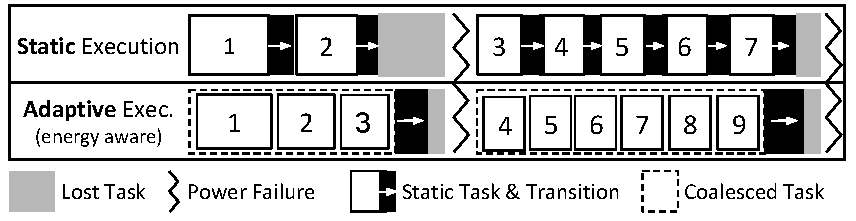
\includegraphics[width=0.5\columnwidth]{figures/coal_Intro_Figure.pdf}
% 	\caption{When $N$ tasks coalesced $N-1$ commit operations are skipped.}
% 	\label{fig:coalIntro}
% \end{wrapfigure}

When a device's buffered energy is sufficient to run multiple consecutive tasks
without a power failure, committing state after each task is an unnecessary
overhead. \sys eliminates this overhead by {\em coalescing} a sequence of
consecutive tasks. \sys coalesces a sequence of tasks by deferring the commit
operations for all tasks to the end of the sequence, performing their commits
as a batch.  In general, committing involves moving state manipulated by a task
into its permanent location in non-volatile main memory.  In particular, \sys's
commit procedure copies dirty pages of memory that a task updated between fast,
volatile working memory and slower, non-volatile main memory; we defer the
details of paging and commit to Section~\ref{sec:memory_virtulaization}.

When \sys coalesces a sequence of $N$ tasks, \sys avoids the cost of commit at
the first $N-1$ boundaries. The first $N-1$ inter-task transitions leave
dirty pages in working memory, deferring the work of committing dirty modified
until the commit of the last task in the sequence.  Coalescing tasks brings a
double benefit. First, coalescing reduces the total number of relatively
high-latency, high-energy non-volatile memory accesses because tasks primarily
access variables in relatively low-latency, low-energy volatile memory.
Second, coalescing eliminates the unnecessary instructions that implement task
commit, which our measurements in Section~\ref{sec:evaluation} show constitute
a substantial run-time overhead.

%it fasten applicaiton exeution be skipping unnecessary data commits operations
%when there is abandond energy. 
 
The effectiveness of coalescing tasks hinges on having an effective {\em
coalescing strategy}, which determines how many consecutive tasks to coalesce.
An effective strategy must be {\em aggressive} enough, attempting to coalesce a
large number of consecutive tasks to amortize a large amount of commit overhead.   
%
If power fails during a long sequence of coalesced tasks, execution will
restart from the last commit, i.e. the first task in the sequence, losing the
progress made by any of the coalesced tasks.
%
An effective strategy must also be {\em
conservative} enough, attempting to coalesce only as many tasks as will execute
to completion using the device's available energy, but no more.
%
An effective coalescing strategy moderates the risk of a power failure during a
long coalesced task and capitalizes on the benefits of deferred commits by
adapting the target size of the dynamic task to the energy available at
runtime. 


%\textcolor{red}{maybe is possible to demonstrate with data? count number of executed non-volatile vs volatile accesses}
%

% % Carlo pseudo code 
% \begin{algorithm}[t]
% 	\caption{Coalescing}
% 	\label{algo:genCoalescing}
% 	\scriptsize
% 	%\small
% 	\begin{algorithmic}[1]
%         \State $H_\text{p} \gets H_\text{c}$
%         \State $H_\text{p} \gets 0$ 
%         \State $B \leftarrow $ \Call{$f_\text{reboot}$}{$B, H_\text{p}$}

%         \While{$\texttt{true}$}
% 	        \State $ B_\text{c} \gets B$
% 	        %
% 	        \While{$ B_\text{c} > 0$}
% 		        \State \Call{execute\_task}{$T_\texttt{i}$}
% 		        \State $W \leftarrow $ \Call{$f_\text{weight}$}{$T_\text{i}$}
% 		        \State $B_\text{c} \gets B_\text{c} - W$
% 				\State $H_\text{c} \gets H_\text{c} + W$
% 	        \EndWhile
% 	        %
% 	         \State $B \leftarrow $ \Call{$f_\text{compl}$}{B, $H_\text{c}$,$H_\text{p}$}
% 	        \State \Call{commit\_to\_fram}{\null}
%         \EndWhile
% 	\end{algorithmic}
% \end{algorithm}
% %
% To describe the proposed strategies we will use the following parameters:
% \begin{itemize}
% \item target budget $B$: total number of static tasks to be coalesced.
% \item current budget $B_\text{c}$: remaining number of tasks to be coalesced before committing to non-volatile memory; 
% \item history $H$: up on reboot, it is the number of executed static tasks between the last two power interrupts. While executing, it is the number of executed static tasks since the last power interrupt.
% \end{itemize}
%
%
% Modifiying Carlo's pseudo code a little 
%\begin{algorithm}[t]
%	\caption{Coalescing}
%	\label{algo:genCoalescing}
%	\scriptsize
%	%\small
%	\begin{algorithmic}[1]
%        \State $B \leftarrow $ \Call{$f_\text{reboot}$}{$H$}
%        \State $H \gets 0$ 
%        \While{$\texttt{true}$}       
%	        \State $ i \gets 0$
%	        %
%	        \While{$ i <= B$}
%		        \State \Call{execute\_task}{$T_\texttt{i}$}
%		        \State $W \leftarrow $ \Call{$f_\text{weight}$}{$T_\text{i}$}
%		        \State $i \gets i + W$
%				\State $H \gets H + W$
%	        \EndWhile
%	        %
%	        \State \Call{commit\_to\_fram}{\null}
%	        \State $B \leftarrow $ \Call{$f_\text{commit}$}{$B$}
%        \EndWhile
%	\end{algorithmic}
%\end{algorithm}

% \begin{wrapfigure}{t}{0.3\textwidth}
\begin{figure}{t}
\fbox{\parbox{\linewidth}{
	\captionof{algorithm}{Coalescing}
	\label{algo:genCoalescing}
	\scriptsize
	%\small
	%
	\begin{algorithmic}[1]
        \State $B \leftarrow $ \Call{$f_\text{reboot}$}{$z$}
        \State $H \gets 0$ 
        \While{$\texttt{true}$}       
	        \State $ i \gets 0$
	        %
	        \While{$ i <= B$}
		        \State \Call{execute\_task}{$T_\texttt{i}$}
		        \State $W \leftarrow $ \Call{$f_\text{weight}$}{$T_\text{i}$}
		        \State $i \gets i + W$
				\State $H \gets H + W$
	        \EndWhile
	        %
	        \State \Call{commit\_to\_fram}{\null}
	        \State $B \leftarrow $ \Call{$f_\text{commit}$}{$B$}
        \EndWhile
	\end{algorithmic}}}
% \end{wrapfigure}
\end{figure}

%	\begin{subfigure}[t]{\linewidth}
%	\end{subfigure}
%
%

\noindent \textbf{Task Coalescing Strategies.} Algorithm~\ref{algo:genCoalescing} shows the general structure of a coalescing strategy. In the algorithm, $B$ (target budget) is total number of static tasks
that \sys will next attempt to coalesce. $T_\text{i}$ is the $i$th task
executed since the last power failure. $H$ (history) is the number tasks
(coalesced or not) executed between the two most recent power failures.
$W_\text{i}$ is the {\em weight} of a task $T_\text{i}$.  A task's weight is an
arbitrary quantity associated with the task that represents its cost in time or
energy to execute; different coalescing strategies may apply different weights
to a task.  For example, a uniform weighting scheme sets the weight of each
task to one, making them all effectively equal in cost to the coalescing
algorithm.  A different policy might use a weighting scheme that sets a task's
weight equal to its run time relative to the task that executes for the
shortest duration, which has unity weight. 

Different coalescing strategies adhere mainly to the template in
Algorithm~\ref{algo:genCoalescing}, varying in only a few {\em characteristic
operations} that the algorithm leaves deliberately abstract.  A strategy's
reboot update function, $f_\text{reboot}$, updates $B$, the target budget,
after a reboot. A strategy's weight lookup function, $f_\text{weight}$, returns
the a task's weight.  A strategy's commit update function, $f_\text{commit}$,
updates $B$ after a successful commit. The following sections detail several
possible coalescing strategies that we developed for \sys. 

\subsubsection{Energy-oblivious Coalescing (EO)}
\label{subsec:energyBlind}

A very simple {\em energy-oblivious} coalescing strategy treats all tasks as
having unity weight and varies the size of a coalesced task linearly. In such a
scheme, the number of tasks to coalesce, $B$, increases by a constant $x$ when
a coalesced sequence of tasks commits, and decreases by the same constant $x$
when a coalesced sequence of tasks fails to complete, i.e., after a power
failure. The characteristic operations of the energy-oblivious strategy are: 


\begin{figure}
    \centering
    \begin{subfigure}[b]{0.49\columnwidth}
        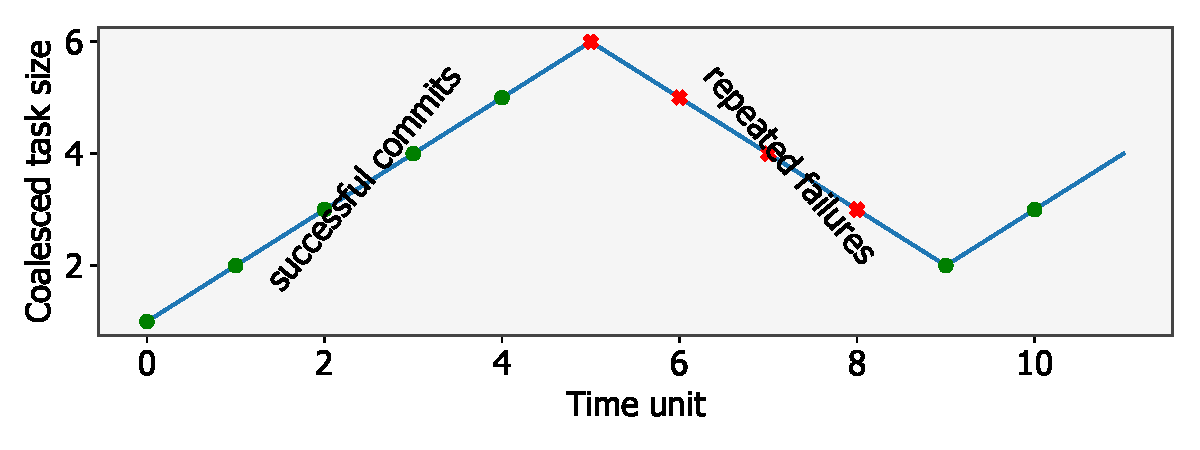
\includegraphics[width=\columnwidth]{figures/slowCoal}
		\caption{The {\em energy-oblivious coalescing} algorithm \emph{linearly} updates its coalescing target.}
		\label{fig:energyBlind}
    \end{subfigure}
    \begin{subfigure}[b]{0.49\columnwidth}
       	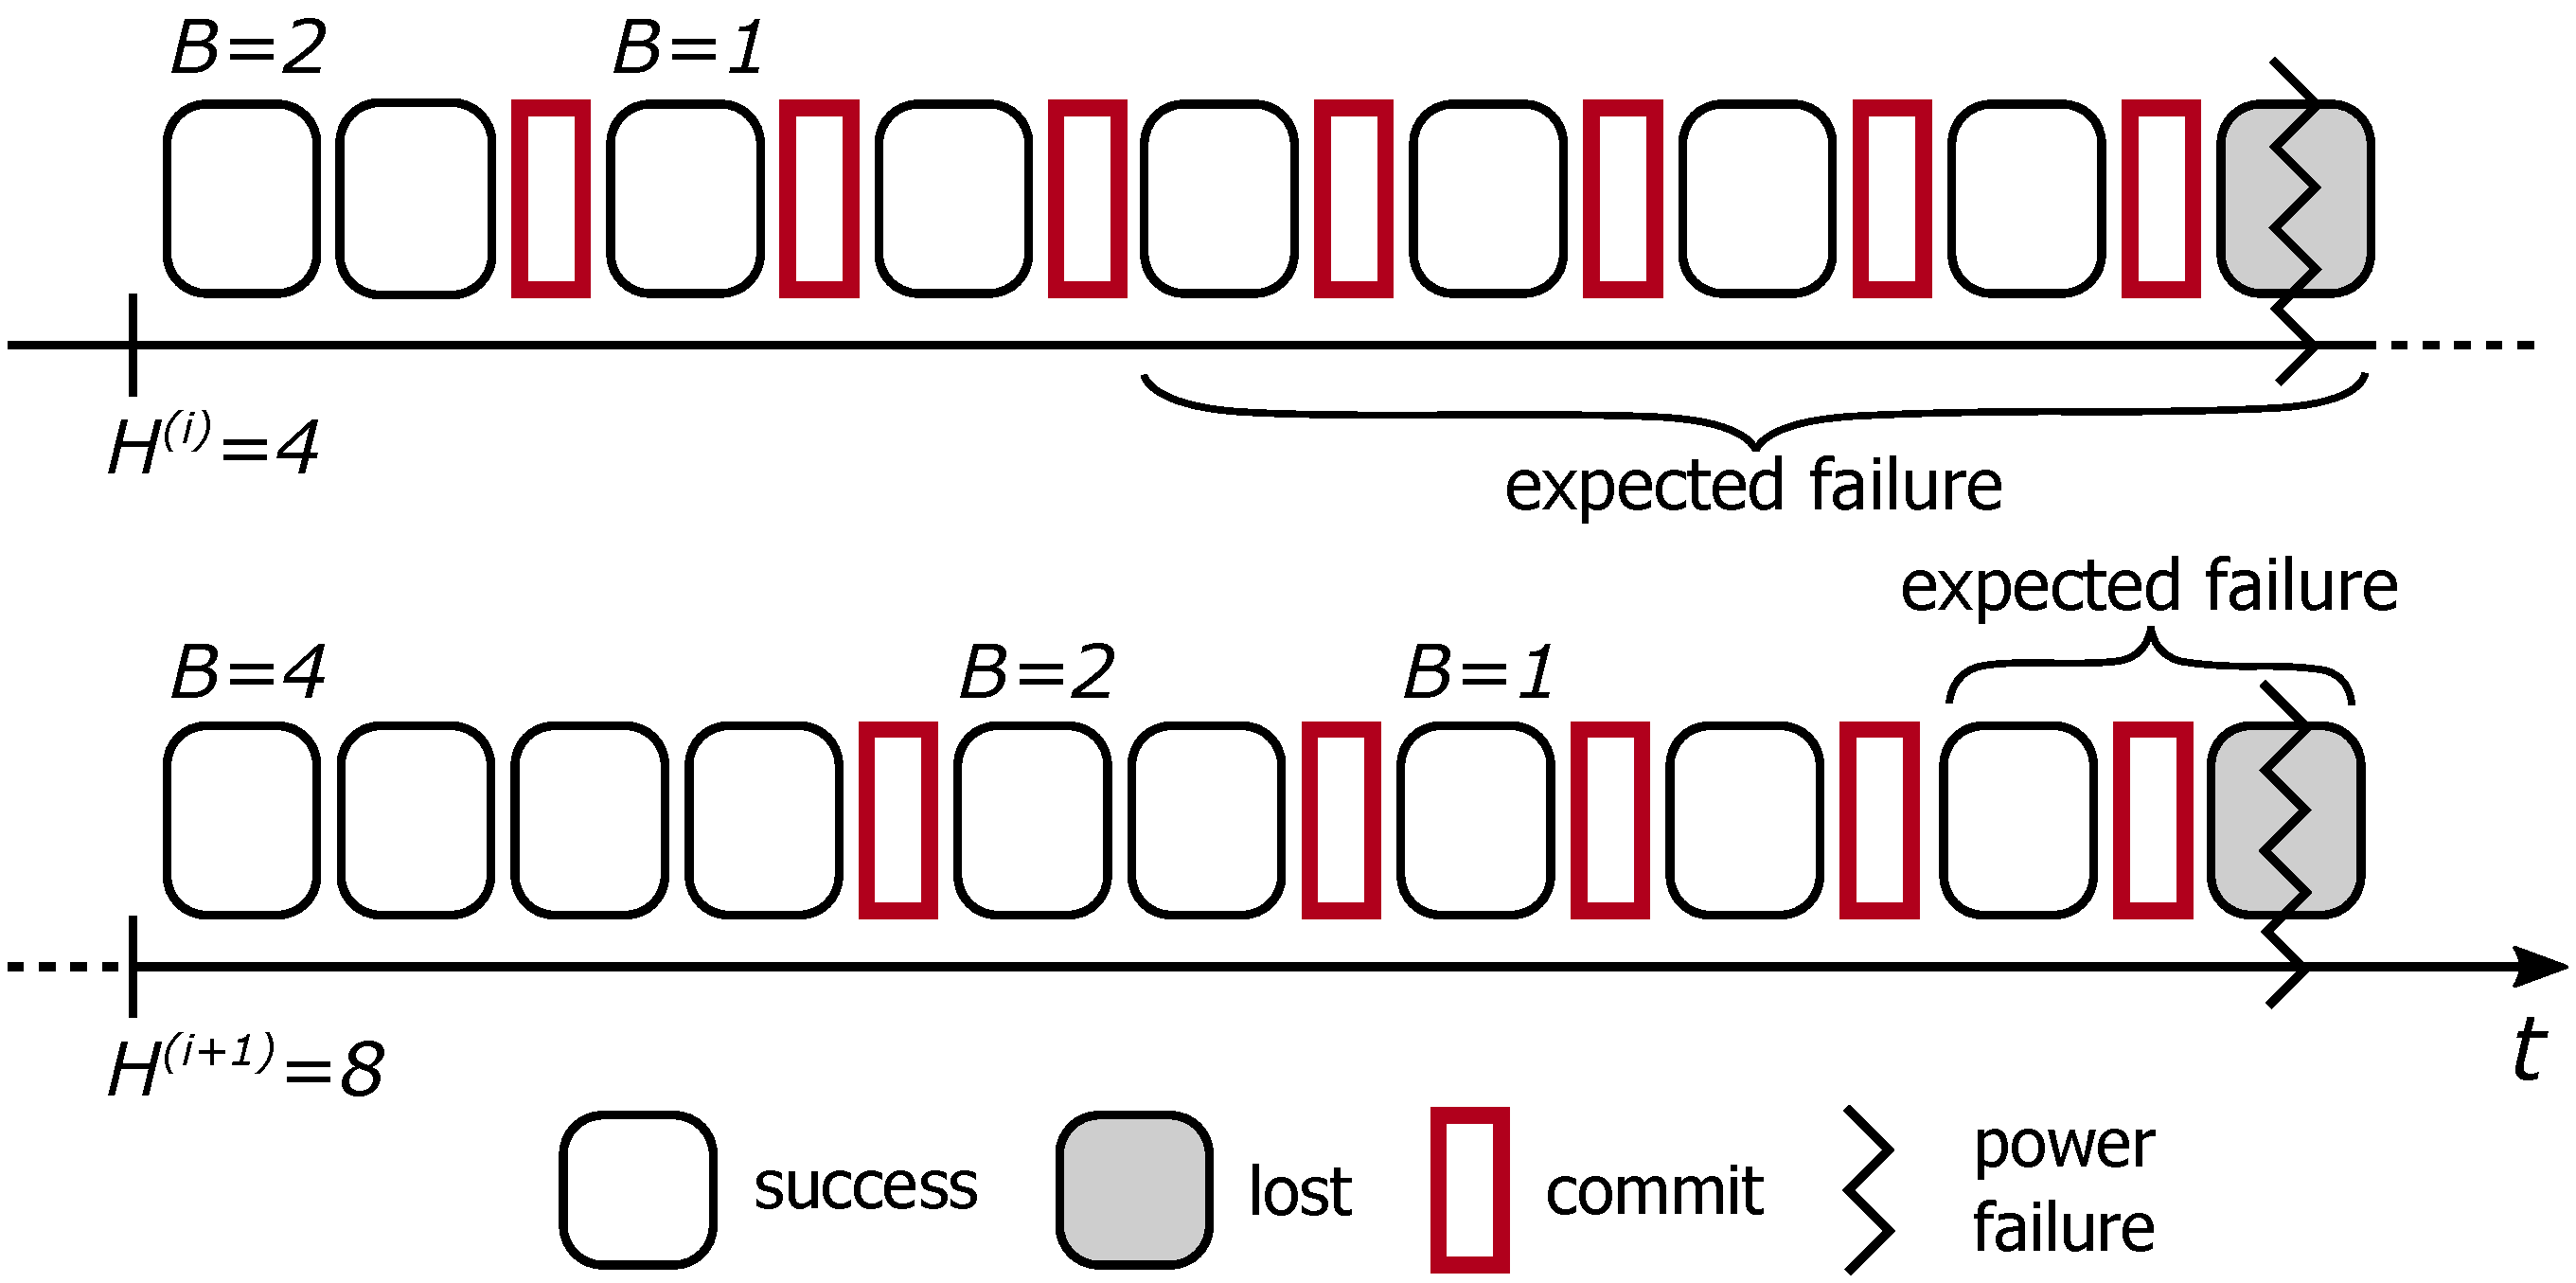
\includegraphics[width=\columnwidth]{figures/energy-aware-coal.pdf}
		\caption{The {\em history-guided coalescing} algorithm uses its recent history of execution to estimate the available amount of energy and set the coalescing target accordingly.}
		\label{fig:energyAware}
    \end{subfigure}
    % \caption{Pictures of animals}\label{fig:animals}
\end{figure}




% % \begin{wrapfigure}{t!}{0.3\textwidth}
% \begin{figure}
% 	\centering
% 	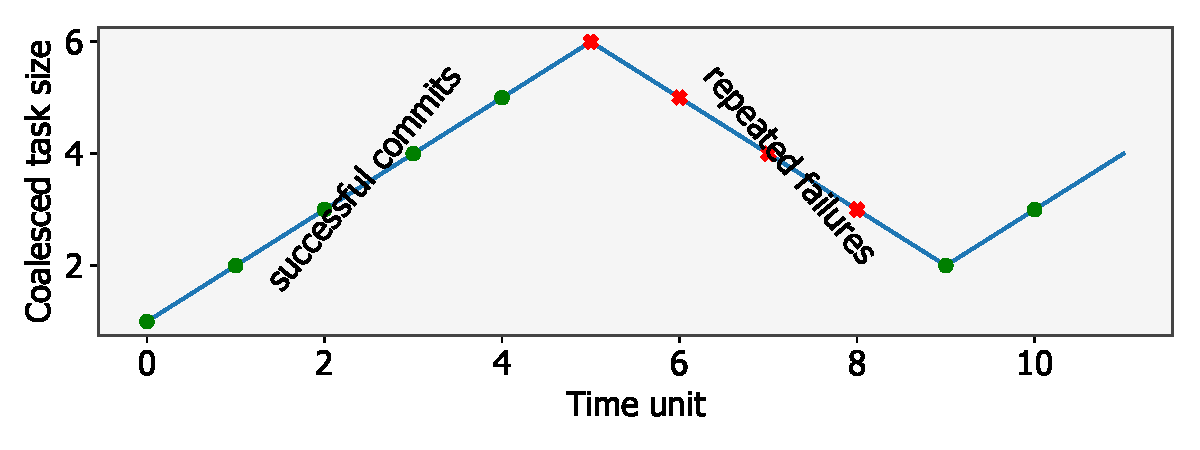
\includegraphics[width=0.48\columnwidth]{figures/slowCoal}
% 	\caption{The {\em energy-oblivious coalescing} algorithm \emph{linearly} updates its coalescing target.}
% 	\label{fig:energyBlind}
% % \end{wrapfigure}
% \end{figure}

% % \begin{wrapfigure}{}{0.5\textwidth}
% \begin{figure}
% 	\centering
% 	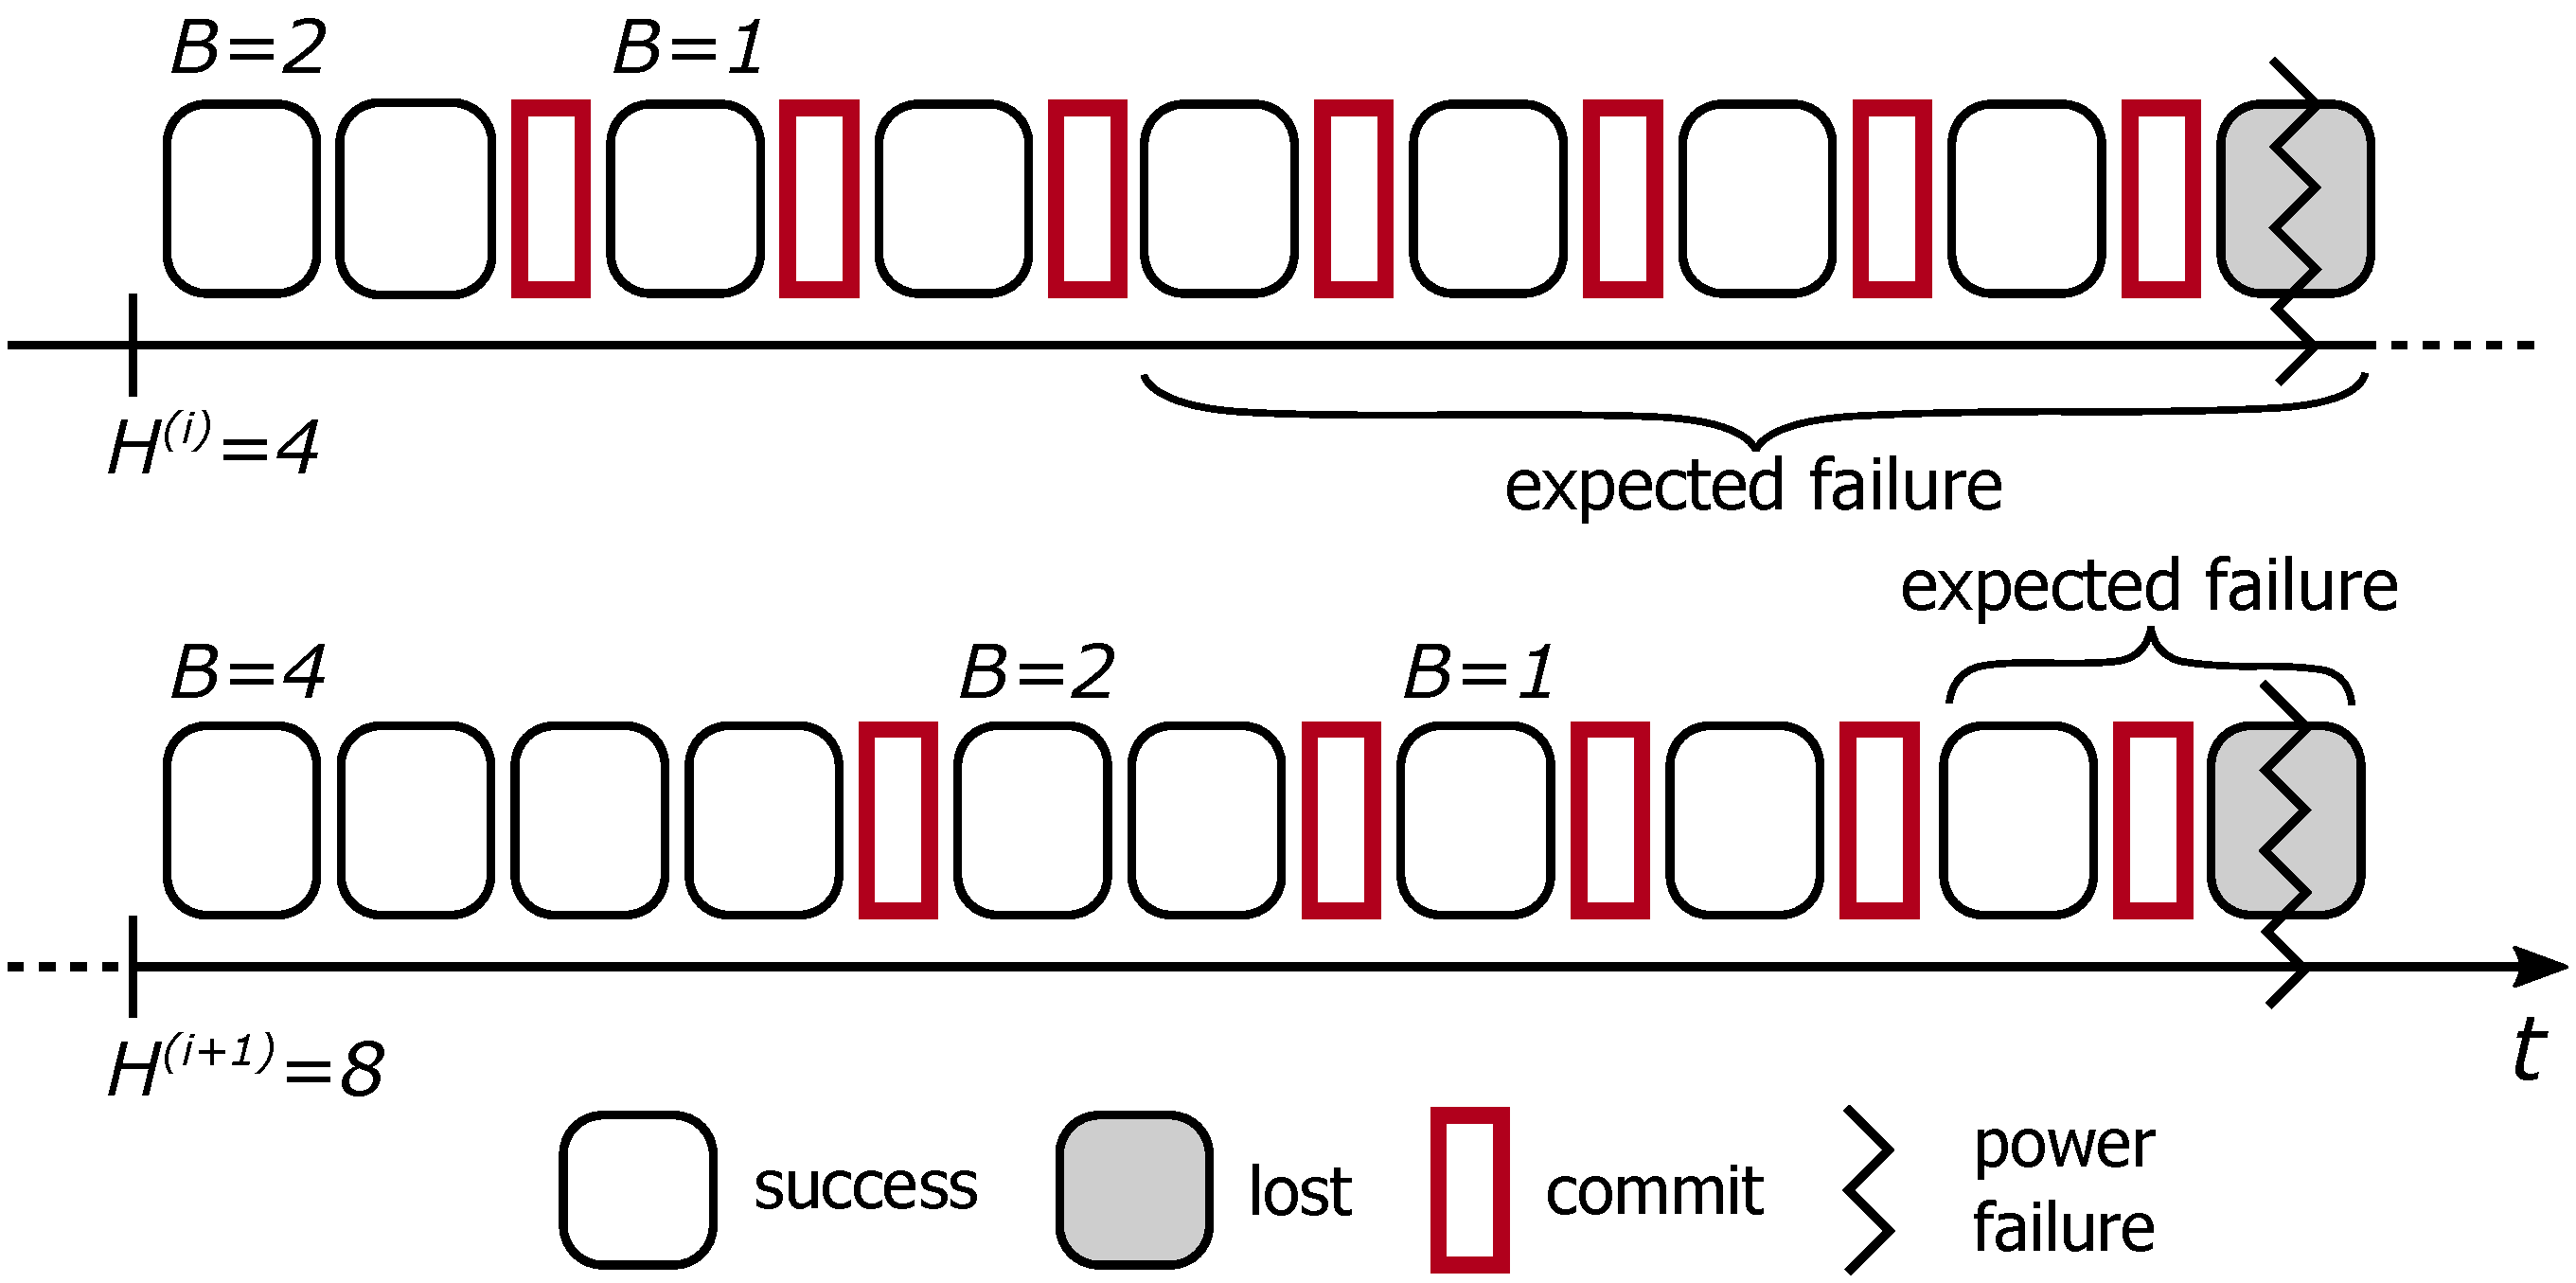
\includegraphics[width=0.48\columnwidth]{figures/energy-aware-coal.pdf}
% 	\caption{The {\em history-guided coalescing} algorithm uses its recent history of execution to estimate the available amount of energy and set the coalescing target accordingly.}
% 	\label{fig:energyAware}
% % \end{wrapfigure}
% \end{figure}

\begin{itemize}
\item $f_\text{reboot}(B) = B - x $;
\item $f_\text{weight}(T_\text{i}) =  1$; 
\item $f_\text{commit}(B) = B + x$; 
\end{itemize}

The energy-oblivious strategy reacts slowly to the variation in the energy
required to execute different tasks and to the variation in the effective quantum of
energy available to the device (i.e., variation in energy buffer size). 
%
Figure~\ref{fig:energyBlind} shows how this strategy may experience a 
large number of repeated power failures without forward progress.
%
With the successful commit of each coalesced task sequence, the coalescing
target increases.  Eventually, the target may be too high and a coalesced task
composed of only fewer tasks will commit without interruption by a power
failure.
%
The strategy then slowly decreases the coalescing target, eventually reaching a
coalescing target that allows completion.
%

A key limitation of this algorithm lies in the equality of the target decrease
in $f_\text{reboot}(B)$ and the increase in $f_\text{commit}(B)$.  If, after
some number $k$ successful commits the target must decrease back to its
original value before the $k$ commits, the algorithm must then decrease $B$ by
$k \times x$.  To accumulate this decrease, this strategy requires $k$ power
failures, after each of which the strategy decreases $B$ by $x$, eventually
decreasing by $k \times x$, but only after a long time. 

\subsubsection{History-Guided Coalescing (HG)}
\label{subsec:energyAware}

\begin{figure*}
    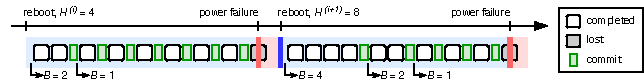
\includegraphics[width=\linewidth]{figures/hg-coal-horiz.pdf}
    \caption{HG coalescing sample execution across two power cycles.}
    \label{fig:hg-coal}
\end{figure*}

The History-Guided (HG) coalescing strategy adapts the coalescing target more
quickly, addressing a key limitation of the EO coalescing strategy.  
%
HG gives each task unity weight, as with EO.  
%
HG differs from EO in how it updates $B$ on commit, and after a power failure.
%
HG assumes that as the duration of execution since a power failure increases,
the amount of energy remaining decreases, and the risk of failing during a long
sequence of coalesced tasks increases.  
%
Consequently, HG decreases the coalescing target by half with each successful commit.
%
HG is {\em history-guided} because it initializes the coalescing target to be
equal to $H$, the total number of tasks executed between the most recent pair
of power failures.
%
While a history of $H$ suggests that there is sufficient energy to coalesce and
successfully commit $H$ tasks (i.e., to set $B = H$), HG conservatively sets $B$ equal to half
of $H$ moderating the risk of a very long coalesced task. 
%
The fraction of the history by which HG adjusts $B$ is arbitrary.
We experimented with a range of fraction values, settling on one half as the
default for HG, because one half had the highest performance. 



The HG algorithm is characterized by the following functions: 

\begin{itemize}
\item $f_\text{reboot}(H) = \lfloor(H / 2)\rfloor;$
\item $f_\text{weight}(T_\text{i}) =  1$; 
\item $f_\text{commit}(B) = \lfloor(B / 2)\rfloor;$ 
\end{itemize}

Figure~\ref{fig:hg-coal} illustrates the operation of the history-guided
coalescing strategy.
The figure shows two power cycles following the $i$th, the latter having an
execution history $H^{(i)} = 4$.
Based on that, $B$ is initially set to two and then decreases to one. Once the
value of $B$ reaches one, HG is, in effect, expecting a power failure,
justifying the conservative approach. After the power failure, HG
uses the most recent history $H^{(i+1)} = 8$ to set $B = 4$
and continue execution.

%, without losing generality or requiring hardware support,
%Moreover, it takes advantage of the guarantees that the energy buffer offers on a fresh start by coalescing many static tasks.

\subsubsection{Weighted History-Guided Coalescing (WHG)}
\label{subsec:energyTaskAware}

The Weighted History-Guided (WHG) coalescing strategy accounts for the
different energy and time cost of a program's tasks when setting the coalescing
target.
%
Each different task in the program consumes a different amount of energy to
execute to completion.  
%
The EO and HG coalescing strategies assume each task has uniform energy cost:
for these strategies, $B$ simply corresponds to a target {\em count} of tasks
coalesced, regardless of the individual cost of each task.
%
However, if one task executes for ten seconds and another executes for one
second, counting tasks misjudges the amount of {\em work} in the coalesced
tasks.

Instead, WHG associates a non-unity weight with each task in the program. 
%
WHG tracks the sum of the weights of tasks in a coalesced sequence of tasks.
%
When the sum of weights reaches $B$, the target, WHG commits the coalesced
task.
%
WHG differs extends EO and HG to explicitly account for the variation in energy
cost of a program's tasks, eliminating the assumption that all tasks do the
same work, which is a key limitation.
%
WHG has the same characteristic operations as HG, except that
$f_\text{weight}(T_\text{i}) = W_\text{i}$.

The effectiveness of the WHG algorithm hinges on correctly identifying the
weight of each task, which WHG assumes is {\em statically} available.
%
Profiling the time and energy cost of tasks in a program is a difficult,
orthogonal problem~\cite{cleancut_2018,baghsorkhi_cgo_2018}.
%
WHG could use the result of an arbitrarily sophisticated profiling procedure.
%
To produce a concrete result in this paper, we give WHG access to a simple
profile of task run time collected offline using a single fixed input.
%
WHG stores the profile in a lookup table that maps a task's identifier to its
weight, making the information available to \sys's scheduler at run time.
